\documentclass[english]{article}
\usepackage[
 %work, %--- activate temporarily to visualise the type area while fine tuning the poster composition
 ,cursor
 ]{KITposter}
 
%Custom packages needed
\usepackage{siunitx}
\usepackage{pgfplots}
\pgfplotsset{compat=newest}
\usepgfplotslibrary{fillbetween}
\usepackage{tikzscale}
\usepackage{tabularx}
\usepackage{enumitem}
\usetikzlibrary{shapes.geometric}
\usetikzlibrary{arrows.meta}

 
\title{Time-Resolved Measurements of Transverse Beam Excitation in an Electron Storage Ring}
\author{\underline{M.-D. Noll}\thanks{marvin-dennis.noll@kit.edu}, E. Bründermann, M. Caselle, E. Huttel, J.~L. Steinmann and A.-S. Müller}
\institute{
\includegraphics[height=6cm]{KARA}}

\footline{\small%
\begin{tabularx}{\linewidth}{p{0.15\linewidth} X p{0.15\linewidth} p{0.09\linewidth}}
     \textbf{Contact} \newline
	 *Marvin-Dennis Noll -- \url{marvin-dennis.noll@kit.edu}\newline Institute for Beam Physics and Technology\newline\url{www.ibpt.kit.edu} \newline Karlsruhe, Germany &
	 \textbf{References} \newline
	 {\footnotesize\begin{enumerate}[nosep,label={[}\arabic*{]}]
	 \item S. Hiramatsu et. al., ``Measurement of Small Beam Size by the Use of SR Interferometer'',\newline in Proc. Particle Accel. Conf., New York, USA, 1999, pp. 492-494
	 \item L. Torino and U. Iriso, ``Transverse beam profile reconstruction using synchrotron radiation interferometry'',\newline \texttt{doi: 10.1103/PhysRevAccelBeams.19.122801}
	 \item B. Kehrer et. al., ``Visible Light Diagnostics at the ANKA Storage Ring''\newline\texttt{doi:10.18429/JACoW-IPAC2015-MOPHA0371}
	 \item M. Patil et al., ``Application of KALYPSO as a diagnostic tool for beam and spectral analysis'',\newline \texttt{doi: 10.18429/JACoW-IPAC2021-WEPAB331}
	 \end{enumerate}} &
	  \textbf{Acknowledgments} \newline 
	  M.-D. Noll acknowledges of the KIT IBPT mechanical engineering department and the mechanical workshop staff" &
	  \textbf{Conference} \newline
	  \raisebox{-4.5cm}{\begin{minipage}[t]{1cm}
\includegraphics[width=8cm]{ibic25.png}\\
	  \textbf{}\end{minipage}}\\
\end{tabularx}
}                  

\def\boxheight{200mm}           
\def\boxsep{5mm}    
\begin{document}
	\maketitle
	\vspace{-40mm}
	
	\begin{boxgrayw}[\boxheight]{Motivation}{}
	\begin{itemize}
		\item Transverse modulation can increase beam size, thus reducing intra-beam scattering
		\item KARA vertical beam size too small for crotch absorber set diffraction limit
		\item Use double slit setup to convert size changes to contrast modulation $V$\textsuperscript{[1, 2]}
		\item Conventionally, $V$ is measured with CMOS camera\textsuperscript{[3]}, $\Rightarrow$ low time resolution
		\item Therefore sample with fast (turn-by-turn) line camera KALYPSO\textsuperscript{[4]} to distinguish mere \textit{position} modulation from desired \textit{size} blow-up
	\end{itemize}
\end{boxgrayw}
\begin{boxgray2w}[\boxheight]{Excitation and Measurement Setup at KARA}{}
	\begin{minipage}{250mm}
		\includegraphics[height=170mm]{img/aufbauModulation.tikz}
	\end{minipage}
	\begin{minipage}{250mm}
		\includegraphics[height=170mm]{img/exSetup.tikz}
	\end{minipage}
\end{boxgray2w}
\vskip\boxsep
\begin{boxgray2w}[\boxheight]{Characterization of the KALYPSO Turn-by-Turn(2.7~MHz) Line Camera}{}
	\begin{minipage}[t]{230mm}
		\includegraphics[height=130mm,width=225mm]{img/kalypsoSpect.tikz}\\
		Response of one pixel to a beam modulation is measured without using the double slit
	\end{minipage}\quad
	\begin{minipage}[t]{230mm}
		\includegraphics[height=130mm,width=225mm]{img/kalypsoSpectrum.tikz}\\
		Spectral response measured with tungsten lamp and set of band-pass filters, averaged over \num{1000} frames and all pixels
	\end{minipage}
\end{boxgray2w}
\begin{boxgrayw}[\boxheight]{Upcoming Upgrades}{}
	\begin{itemize}
		\item Experiments show double slit measurements not possible due to (radiation-) damaged optics
		
		\vspace{5mm}
		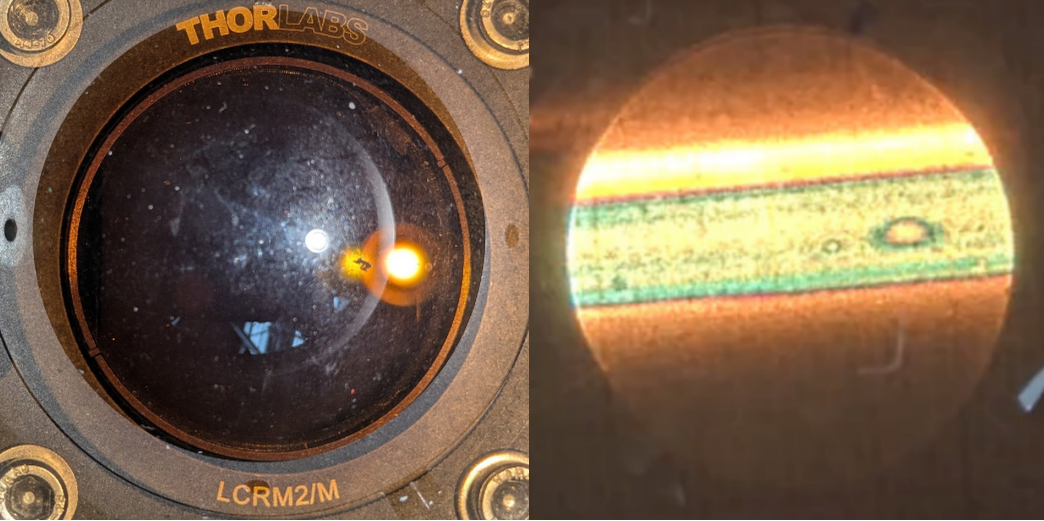
\includegraphics[width=145mm]{img/mirrorAndWindow.png}
		\item Mirror and windows are to be replaced by new components
		\item Old green bandpass filter is switched for NIR filter
	\end{itemize}
\end{boxgrayw}
\vskip\boxsep
\begin{boxgrayw}[\boxheight]{Double Slit}{}
	\includegraphics[height=175mm,width=220mm]{img/ds.tikz}
\end{boxgrayw}
\begin{boxgrayw}[\boxheight]{Inverted Double Slit}{}
	\includegraphics[height=175mm,width=220mm]{img/dsInverted.tikz}
\end{boxgrayw}
\begin{boxgrayw}[\boxheight]{Summary and Outlook}{}
	\begin{itemize}
		\item Feasibility of setup shown, however limited by the low-light conditions
		\item Characterizations of KALYPSO show spectral response similarity to CMOS camera
		\item Other geometries than the double slit, e.g. an inverted version, are studied
		\item After KALYPSO setup is in operation, systematical studies of different accelerator operation modes(injection, energy ramp, ...) will be done
	\end{itemize}
\end{boxgrayw}
	
\end{document}
